\subsection{Methods for Structured Features}
\label{sec:methods.structured}

% Author: Flo

Other than Flat Features, Structured Features are features where a certain
underlying structure is known or assumed and will be used. This approach tends
to outperform Methods for Flat Features in certain cases, for example
genome analysis in bio-informatics (\cite{Tang:14}).

Methods for Structured Features can be categorized into $3$ groups:

\begin{itemize}
  \item Graph Methods
  \item Tree Methods
  \item Group Methods
\end{itemize}

The decision which structure to use, is dependent on the relationship of the
features. Group and tree methods basically assume simple hierarchical groupings
of features, whereas graph methods build a more complex relationship-graph.

\subsubsection{Group Methods}
\label{sec:methods.structured.group}

% Author: Flo
  
Since it is often useful to select or discard a group of features at once,
features can be grouped into feature-groups. Weights can now be assigned to
whole groups by minimization techniques and groups with weights close to $0$ can be
eliminated. An algorithm that uses this approach is the Group Lasso. 

This approach does not necessarily exclude the possibility to select single
features inside feature groups as well. As a matter of fact some methods
(e.g. the Sparse Group Lasso Regularization) perform feature-group selection and
feature selection at once (\cite{Tang:14}).

\begin{figure}[!ht]
  \centering 
  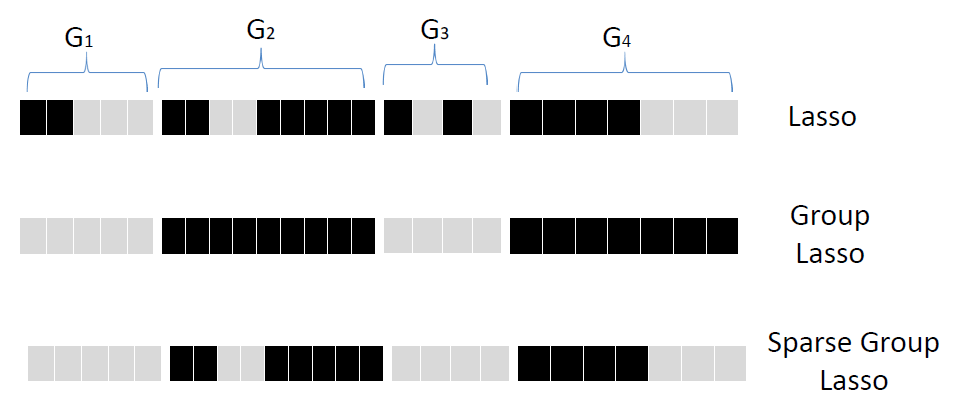
\includegraphics[width=0.8\textwidth]{chapters/methods/structured/group_lasso}
  \caption{Reprinted from \cite{Tang:14}. Illustration of Lasso, Group Lasso
  and Sparse Group Lasso.
  Features can be grouped into 4 disjoint groups {G1,G2,G3,G4}. Each cell denotes a feature and light color
represents the corresponding cell with coefficient zero (\cite{Tang:14}).}
  \label{fig:methods.structured.group.lasso}
\end{figure}

In Figure \ref{fig:methods.structured.group.lasso} an example is given of
how Lasso, Group Lasso and Sparse Group Lasso would behave in comparison
to each other when selecting features. 

Sometimes the given data structure might suggest overlapping feature-groups,
where a feature can belong to more than one group. This case is no longer
handled correctly by the Sparse Group Lasso-method. Some methods that handle
this scenario are:

\begin{itemize}
  \item \cite{Liu:10}
  \item \cite{Kim:10}
  \item \cite{Jenatton:10}
  \item \cite{Jacob:09}
\end{itemize}






\subsubsection{Tree Methods}
\label{sec:methods.structured.tree}

% Author: Flo

With Tree Methods, features are assumed to have a certain structure, where
features can be grouped into groups, and these groups can again be grouped into
groups, until there is only one group left.

This index-tree-structure can be visualized as tree, with all features being
leafes (see Figure \ref{fig:methods.structured.tree.lasso}).

\begin{figure}[!ht]
  \centering 
  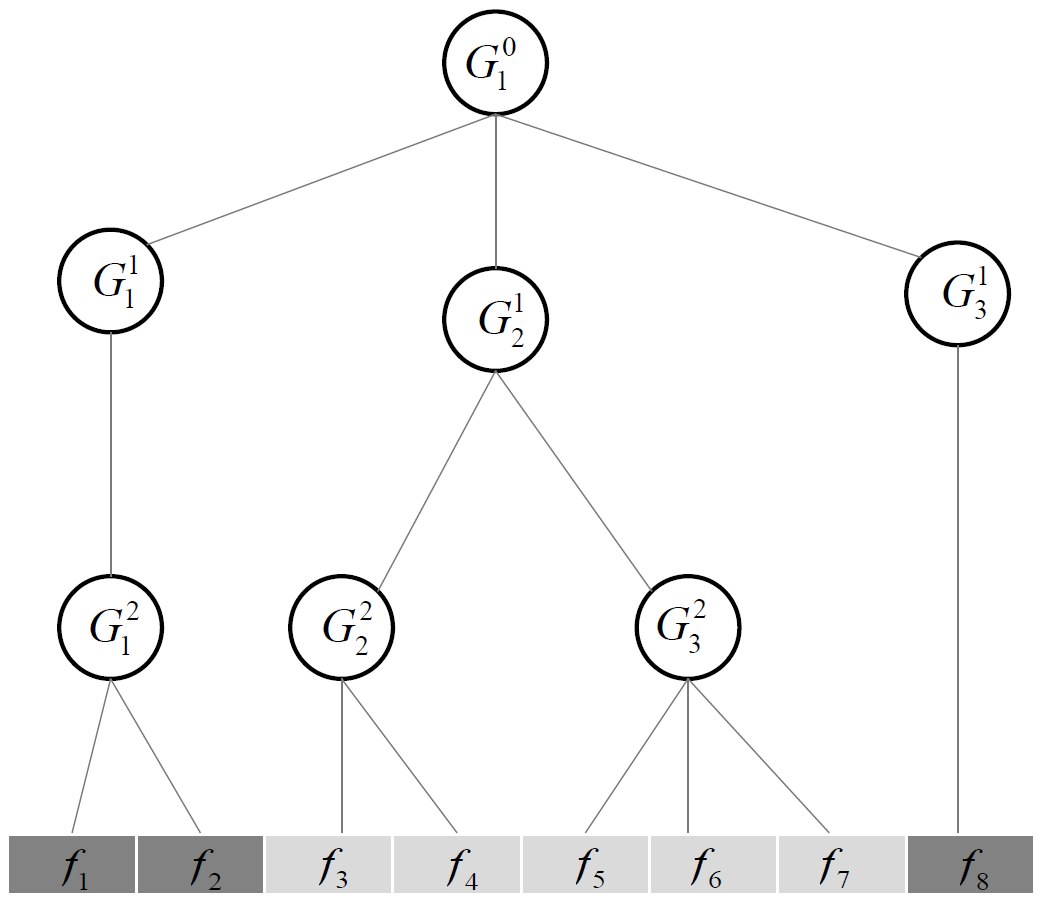
\includegraphics[width=0.5\textwidth]{chapters/methods/structured/tree_lasso}
  \caption{Reprinted from \cite{Tang:14}. Illustration of an index tree.
  E.g. Features $f_1$ and $f_2$ can be grouped into $G_1^2$ (\cite{Tang:14}).}
  \label{fig:methods.structured.tree.lasso}
\end{figure}

Using index-trees, methods like the tree structured group Lasso (\cite{Kim:10})
can use this structure to eliminate tree-nodes on a higher level of the hierachy and
therefore eliminate many features at once.
\subsection{Graph Methods}
\label{sec:methods.structured.graph}

% Author: Flo
  